\documentclass[tikz]{standalone}
\usepackage{pgfplots}
\pgfplotsset{compat=1.15}
\usepackage{mathrsfs}
\usetikzlibrary{arrows,calc}
\usepackage{tkz-euclide}

\pagestyle{empty}

\definecolor{AngleClr}{rgb}{0,0.39215686274509803,0}
\definecolor{ShapeClr}{rgb}{0.6,0.2,0}

\begin{document}

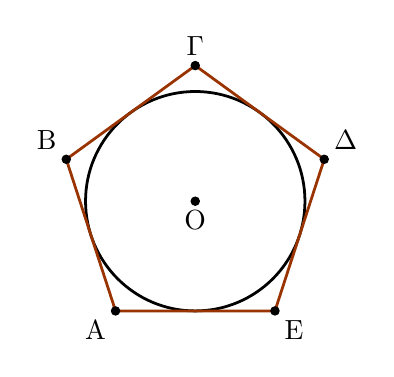
\begin{tikzpicture}[scale=.75]
\tkzSetUpLine[line width=1pt,color=black]
\tkzSetUpPoint[fill=black]

\tkzDefPoints{0/0/P0,2.7/0/P1}

\tkzDefRegPolygon[side,sides=5](P0,P1)
\tkzDefMidPoint(P1,P2) \tkzGetPoint{M}


\tkzFillPolygon[fill=white](P1,P2,P3,P4,P5)

\tkzDefCircle[circum](P1,P2,P3) \tkzGetPoint{O}

\tkzDrawCircle[line width=1pt,black](O,M)

\tkzDrawPolygon[color=ShapeClr](P1,P2,P3,P4,P5)
\tkzDrawPoints[size=3](P1,P2,P3,P4,P5,O)
\tkzLabelPoint[below left](P1){$\rm A$}
\tkzLabelPoint[below right](P2){$\rm E$}
\tkzLabelPoint[above right](P3){$\rm \Delta$}
\tkzLabelPoint[above](P4){$\rm \Gamma$}
\tkzLabelPoint[above left](P5){$\rm B$}

\tkzLabelPoint[below](O){$\rm O$}

\end{tikzpicture}

\end{document}
